% !TEX program = xelatex
% coding=utf-8
\documentclass[14pt]{Bredelebeamer}
\usepackage{ctex}
%\usepackage{beamerthemesplit}
\usepackage{fontawesome}
\usepackage{multirow}
\usepackage{booktabs}
\usepackage{graphicx}
%\usepackage[framemethod=tikz]{mdframed}
\usepackage{tikz}
\usepackage{epstopdf}
\usetikzlibrary{arrows,decorations.markings}
\usetikzlibrary{decorations.pathreplacing}
\usetikzlibrary{calc}
\renewcommand{\today}{2016 年 6 月 14 日}
 \setbeamerfont{title}{size=\LARGE}
 \setbeamerfont{subtitle}{size=\LARGE}

%%%%%%%%%%%%%%%%%%%%%%%%%%%%%%%%%%%%%%%%%%%%%%%%



\title[本科毕设]{基于SVM的LSB信息隐藏算法研究与优化}
\subtitle{The Study and Improvement of SVM-based LSB Steganography}
\author[扬州计划]{李欣宜}
\institute[]{大连理工大学}
\date{\faCalendar{ } 2016 年 6 月 13 日}
\subject{毕业设计}

\begin{document}

\begin{frame}
  \titlepage
\end{frame}

\begin{frame}{概览}
  \begin{columns}
    \begin{column}{.5\textwidth}
        \tableofcontents
    \end{column}
  \end{columns}
\end{frame}

\section{选题背景}
\begin{frame}{题目来源}
  论文题目《基于SVM的LSB信息隐藏算法研究与优化》为自拟课题。
  \begin{alertblock}{LSB隐写术(LSB Steganography)}
    \begin{itemize}
      \item 最早接触隐写术的概念在《密码学》课堂上
      \item 因为感兴趣曾经使用Wolfram Mathematica实现了基本的隐写程序,并写入了博客(\faChain \url{https://www.yangzhou301.com/2015/11/15/861014670/})
    \end{itemize}
  \end{alertblock}
  \begin{block}{支持向量机(SVM)}
    \begin{itemize}
      \item 机器学习是现在非常流行的研究方向,可以在很多领域实现优化
      \item 完成过SVM相关的实战(\faChain \url{https://github.com/Lixinyi-DUT/machine_learning_techniques})
    \end{itemize}
  \end{block}
  所以在毕设中尝试完成应用SVM针对LSB图像隐写进行优化。
\end{frame}

\subsection{研究背景}
\begin{frame}{隐写术}

{\large
隐写是指把一个文件、消息、图像或者视频隐藏到另一个文件、消息、图像或者视频的行为。与密码学不同的是,隐写术旨在隐藏消息或其他形式的信息本身的\alert{存在},不引起发送方和接收方以外的人的怀疑而完成信息的交流,而密码学则用于隐藏这些信息的\alert{内容},使得非发送方或接收方即使截获消息也无法得到所交流的信息的真实内容。
必须满足条件:
\begin{itemize}
  \item	保密性
  \item 可获得性
  \item 完整性
\end{itemize}
}
\end{frame}

\section{LSB隐写实现和缺陷分析}
\subsection{LSB隐写研究}
\begin{frame}{LSB图像隐写}
\begin{description}
  \item[秘密消息] 需要隐藏的信息
  \item[载体cover] 用来隐藏信息的文件,多媒体文件因为包含的数据巨大,适合作为载体。在本文中选择像素图像为载体。
  \item[伪装stego] 隐藏了秘密消息的文件,与载体图像看上去没有区别
  \item[最低有效位LSB] 数据的最低位,对于8位二进制为第0位
\end{description}
\begin{alertblock}<3->{秘密消息}
  `a' = 0b\textcolor<4>{alertTitleBlockColor}{01100001}
\end{alertblock}

\begin{table}
  \begin{tabular}{c|c c c c c c c c}
    像素值 & 7 & 6 & 5 & 4 & 3& 2& 1& 0 \\
    \hline
    \only<2-3>{\textcolor{exampleTitleBlockColor}{226}}
    \only<4>{\textcolor{alertTitleBlockColor}{226}} & 1 & 1 & 1 & 0 & 0 & 0 & 1 &\only<2-3>{\textcolor{exampleTitleBlockColor}{0}} \only<4>{\textcolor{alertTitleBlockColor}{0}}\\
    \only<2-3>{\textcolor{exampleTitleBlockColor}{136}} \only<4>{\textcolor{alertTitleBlockColor}{137}}& 1 & 0 & 0 & 0 & 1 & 0 & 0 & \only<2-3>{\textcolor{exampleTitleBlockColor}{0}} \only<4>{\textcolor{alertTitleBlockColor}{1}}\\
    \only<2-3>{\textcolor{exampleTitleBlockColor}{124}} \only<4>{\textcolor{alertTitleBlockColor}{125}}& 0 & 1 & 1 & 1 & 1 & 1 & 0 & \only<2-3>{\textcolor{exampleTitleBlockColor}{0}} \only<4>{\textcolor{alertTitleBlockColor}{1}}\\
    \only<2-3>{\textcolor{exampleTitleBlockColor}{226}} \only<4>{\textcolor{alertTitleBlockColor}{226}}& 1 & 1 & 1 & 0 & 0 & 0 & 1 & \only<2-3>{\textcolor{exampleTitleBlockColor}{0}} \only<4>{\textcolor{alertTitleBlockColor}{0}}\\
    \only<2-3>{\textcolor{exampleTitleBlockColor}{137}} \only<4>{\textcolor{alertTitleBlockColor}{136}}& 1 & 0 & 0 & 0 & 1 & 0 & 0 & \only<2-3>{\textcolor{exampleTitleBlockColor}{1}} \only<4>{\textcolor{alertTitleBlockColor}{0}}\\
    \only<2-3>{\textcolor{exampleTitleBlockColor}{124}} \only<4>{\textcolor{alertTitleBlockColor}{124}}& 0 & 1 & 1 & 1 & 1 & 1 & 0 & \only<2-3>{\textcolor{exampleTitleBlockColor}{0}} \only<4>{\textcolor{alertTitleBlockColor}{0}}\\
    \only<2-3>{\textcolor{exampleTitleBlockColor}{223}} \only<4>{\textcolor{alertTitleBlockColor}{222}}& 1 & 1 & 0 & 1 & 1 & 1 & 1 & \only<2-3>{\textcolor{exampleTitleBlockColor}{1}} \only<4>{\textcolor{alertTitleBlockColor}{0}}\\
    \only<2-3>{\textcolor{exampleTitleBlockColor}{137}} \only<4>{\textcolor{alertTitleBlockColor}{137}}& 1 & 0 & 0 & 0 & 1 & 0 & 0 & \only<2-3>{\textcolor{exampleTitleBlockColor}{1}} \only<4>{\textcolor{alertTitleBlockColor}{1}}\\
  \end{tabular}
\end{table}

\end{frame}

\begin{frame}{LSB图像隐写的实现}
    \begin{figure}
      \centering
      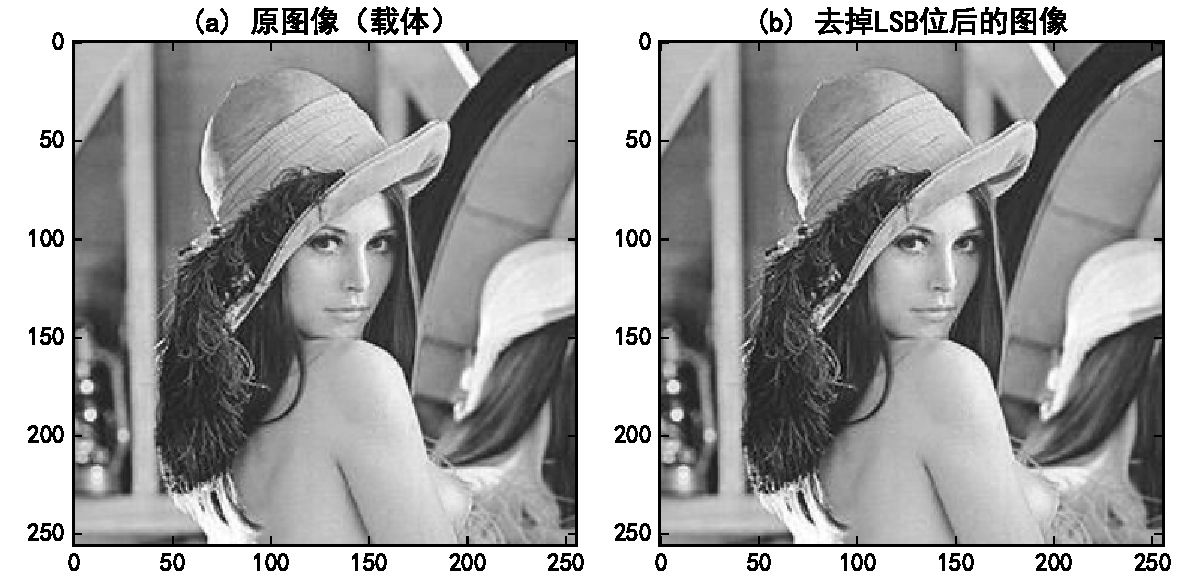
\includegraphics[width=.9\textwidth]{images/demo1}
    \end{figure}
    \begin{alertblock}{8bit灰度图像截去LSB平面前后无明显变化}
      图像的LSB平面的变化不会带来强烈的视觉变化
    \end{alertblock}
\end{frame}

\begin{frame}{LSB图像隐写的实现}
  \begin{block}{顺序嵌入}
    先将秘密消息的长度$l$转化为二进制数嵌入在图像的前$n$位,再按照图像的自然顺序将秘密消息逐个嵌入接下来的像素
  \end{block}
  \begin{figure}
    \centering
    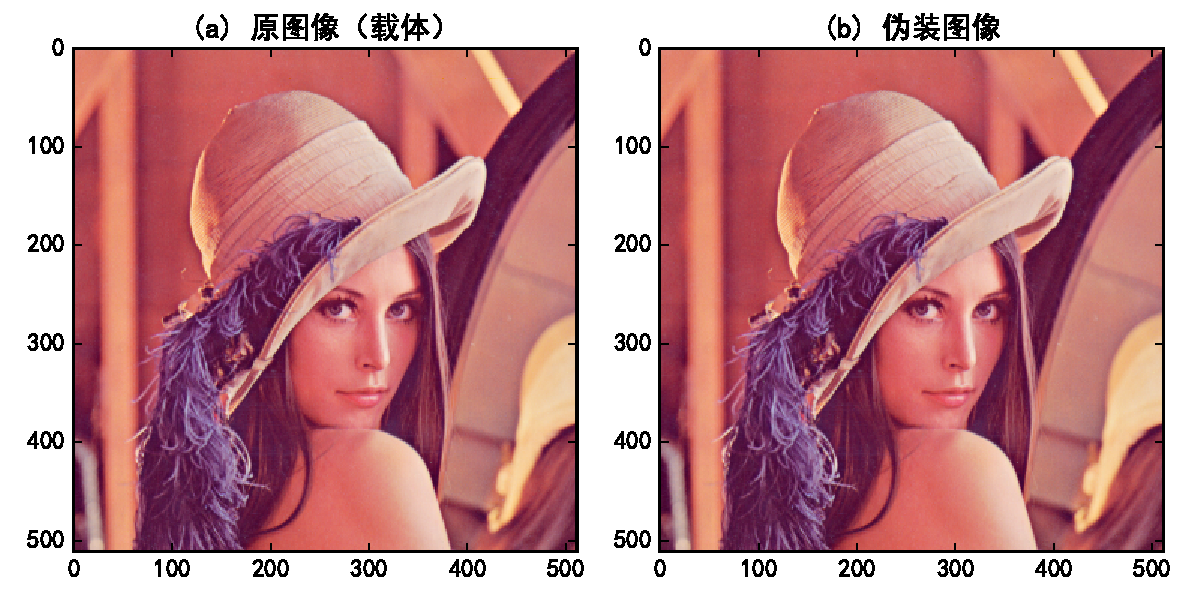
\includegraphics[width=.7\textwidth]{images/gettys}
    %\caption{隐写了《葛底斯堡演说》全文前后的LENA图}
  \end{figure}
  \begin{exampleblock}{消息提取}
    先提取前$n$个像素的LSB位获得消息长度$l$,再读取接下来的$8l$个像素的LSB位恢复完整的消息
  \end{exampleblock}
\end{frame}

\subsection{隐写分析}

\begin{frame}{隐写分析}
  \begin{columns}
    \begin{column}{.25\textwidth}
      \begin{block}{}
        \begin{itemize}
          \item 视觉隐写分析
          \item 结构隐写分析
          \item 统计隐写分析
          \item 学习隐写分析
        \end{itemize}
      \end{block}
    \end{column}
    \begin{column}{.7\textwidth}
      \begin{figure}
        \centering
        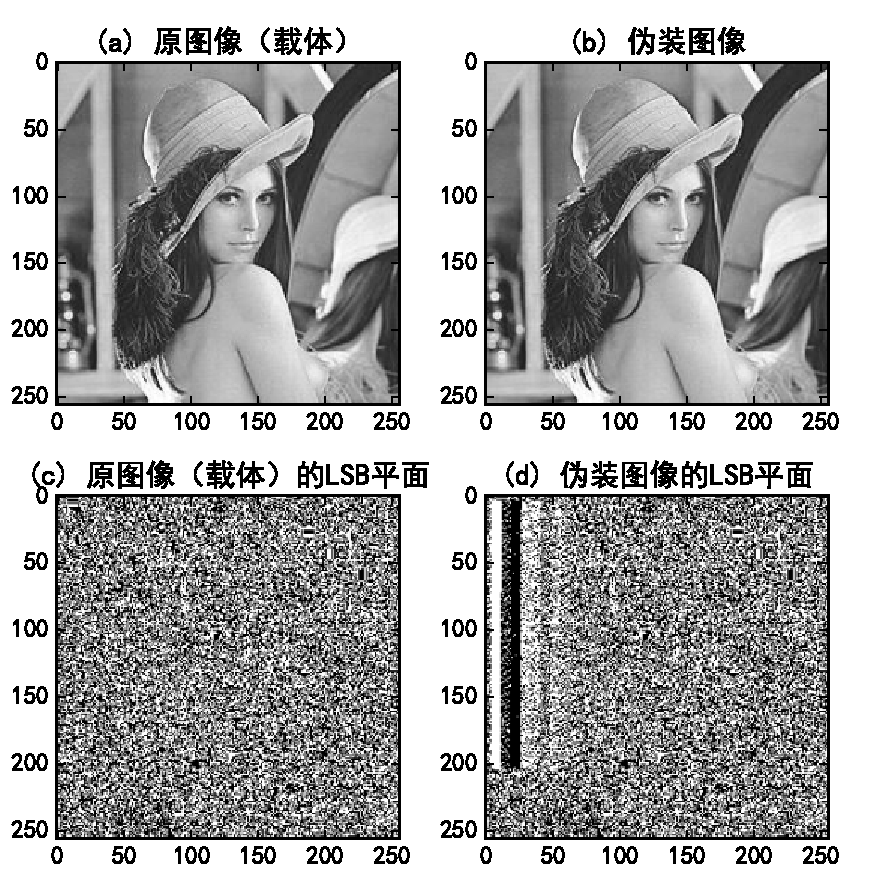
\includegraphics[width=.95\textwidth]{images/lsb1}
      \end{figure}
    \end{column}
  \end{columns}
\end{frame}



\begin{frame}{秘钥隐写系统}
\begin{block}{引入秘钥的隐写系统}
  将秘钥作为PRNG的种子,确定隐藏的像素序列
\end{block}

  \begin{tikzpicture}[decoration={
    markings,
    mark=at position 1 with {\arrow[scale=2]{angle 90}};
  },scale=0.33]
\path(5,15) node(A) {\bf{发送方}};
\path(25,15) node(B) {\bf{接收方}};
{\footnotesize
{\color<8>{normalTitleBlockColor}\path  (0,6) node(M1) [label=below:秘密消息]{
\includegraphics[scale=.07]{icons/email}};}

\path  (0,0) node(C) [label=below:载体] {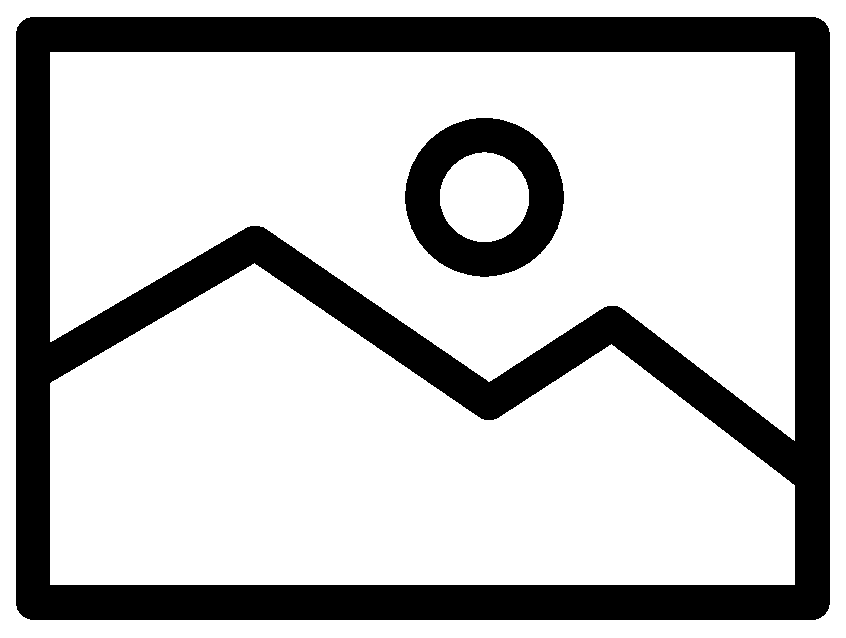
\includegraphics[scale=.04]{icons/landscape-image}};

\path<9->  (5,10) node(K1) [label=above:秘钥]{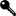
\includegraphics[scale=.07]{icons/house-door-key}};
\path<9->  (25,10) node(K2) [label=above:秘钥]{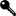
\includegraphics[scale=.07]{icons/house-door-key}};
{\color<8>{normalTitleBlockColor}\path<7->  (30,3) node(M2) [label=below:秘密消息]{
\includegraphics[scale=.07]{icons/email}};}
{\color<5>{normalTitleBlockColor} \path<3->  (10,3) node(S1) [label=below:伪装图像] {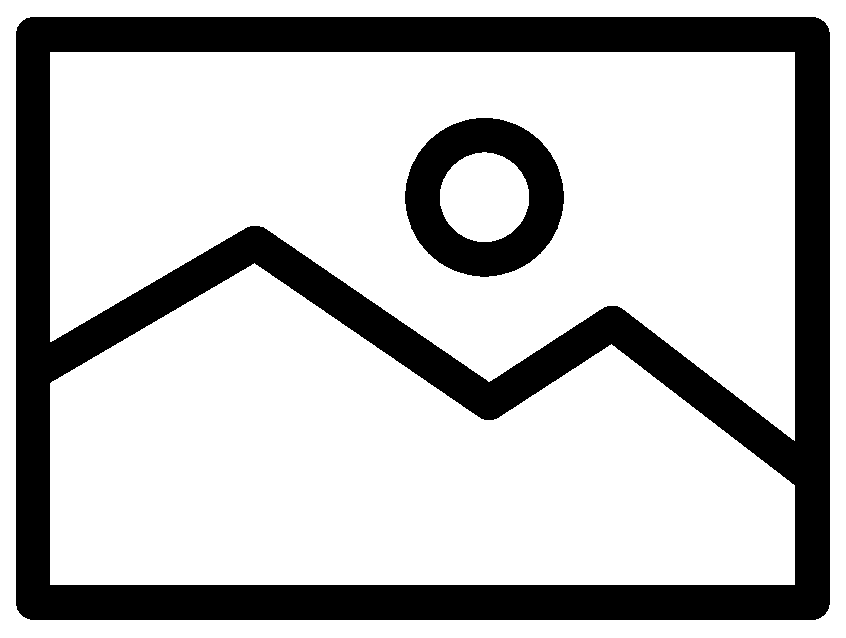
\includegraphics[scale=.04]{icons/landscape-image}};}
{\color<5>{normalTitleBlockColor} \path<5->  (20,3) node(S2) [label=below:伪装图像] {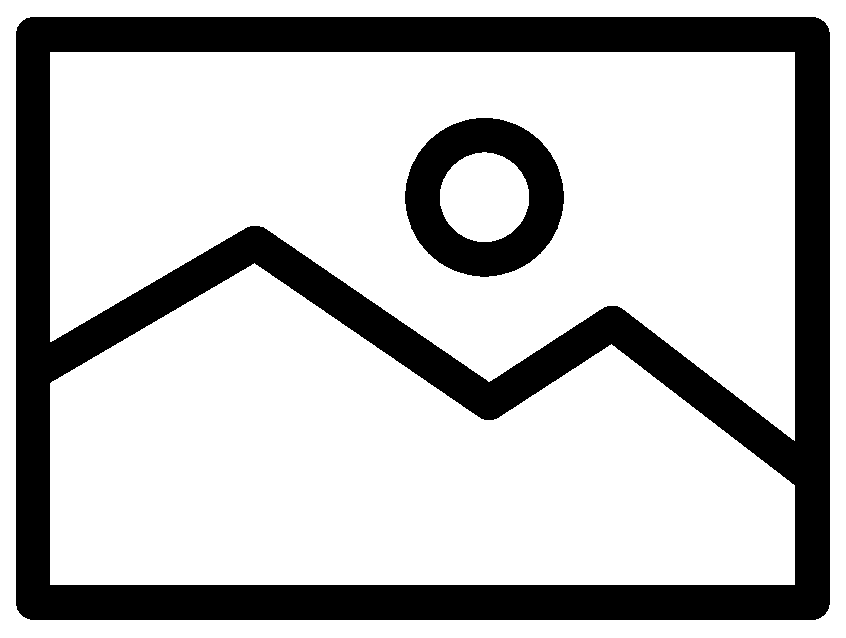
\includegraphics[scale=.04]{icons/landscape-image}};}
\draw<2-> (3.5,2.1) rectangle node(P1)[align=center] {嵌入消息\\(隐写)} (6.5,3.9);
\draw<6-> (23.5,2.1) rectangle node(P2)[align=center] {提取消息\\(恢复)} (26.5,3.9);
{\color<10>{normalTitleBlockColor} \draw<4-> (13.4,2.5) rectangle node(CH1) {公共信道}
(16.6,3.5);}
{\color<10>{alertTextColor} \draw<9-> (13.4,9.5) rectangle node(CH2) {安全信道}
(16.6,10.5);}
\draw<2->[->,thick] (C) -- (3.4,2.5);
\draw<2->[->,thick] (M1) -- (3.4,3.5);
\draw<9->[->,thick] (K1) -- (5,4);
\draw<3->[->,thick] (6.6,3) -- (S1);
\draw<4->[->,thick] (S1)--(13.3,3);
\draw<5->[->,thick] (16.7,3)--(S2);
\draw<6->[->,thick] (S2) -- (23.4,3);
\draw<7->[->,thick] (26.6,3) -- (M2);
\draw<9->[<->,thick] (K1)--(13.3,10);
\draw<9->[<->,thick] (16.7,10)--(K2);
\draw<9->[->,thick] (K2)--(25,4);
\draw[line width=2,dashed,dash pattern=on 6pt off 4pt,color=gray] (-2,-2) rectangle  (12,13);
\draw[line width=2,dashed,dash pattern=on 6pt off 4pt,color=gray] (18,-2) rectangle  (32,13);
}

\end{tikzpicture}
\end{frame}

\begin{frame}{针对LSB的图像隐写分析}
  \begin{itemize}
    \item 秘钥隐写系统对双方的通信资源要求较高
    \item 存在可以攻破随机位置隐写的LSB图像分析方法
      \end{itemize}
    \begin{block}{经典的LSB图像分析方法}

      本文中实现了这些方法用于评估伪装图像的安全性
  \begin{itemize}
    \item $\chi^2$检测
    \item 样本对分析(SPA)
    \item RS隐写分析
  \end{itemize}
    \end{block}
\end{frame}

\begin{frame}{$\chi^2$检测}
  \subtitle{值对分析:伪装图像的直方图中存在更多大致等高的像素值对}
  \begin{figure}
    \centering
    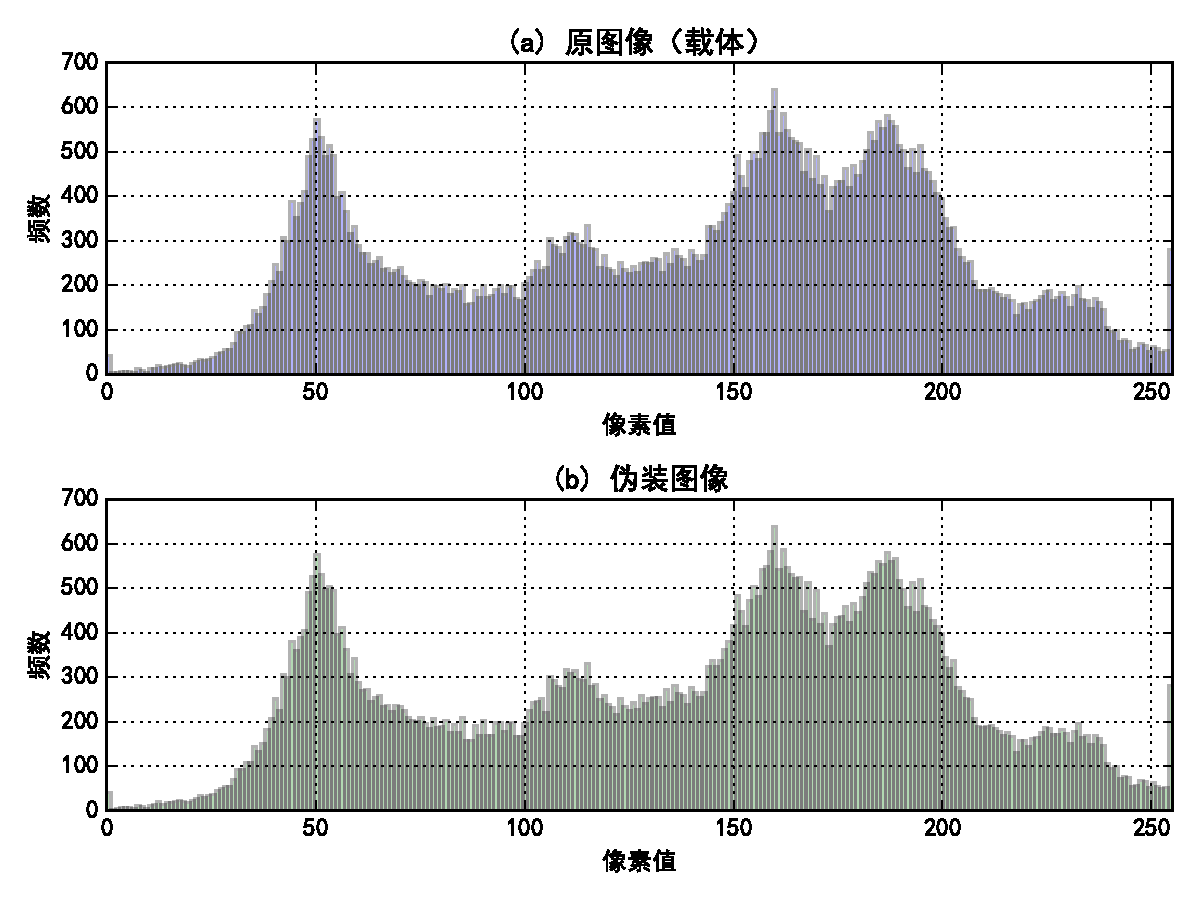
\includegraphics[width=.9\textwidth]{images/hist2}
  \end{figure}
\end{frame}

\begin{frame}{$\chi^2$检测}
  \begin{exampleblock}{原理}
  由于LSB修改的过程实际可用看做像素值$2i$与$2i+1$间的变换,相比自然图像,秘密消息的嵌入使得值对$\left( 2i , 2i+1\right)$间的分布更接近均匀分布。
\end{exampleblock}

\begin{block}{实现方法}
  计算
  $${S_{PoV}} = \sum\limits_{i = 0}^{127} {\frac{{{{\left[ {{h_{2i}} - \frac{1}{2}\left( {{h_{2i}} + {h_{2i + 1}}} \right)} \right]}^2}}}{{\frac{1}{2}\left( {{h_{2i}} + {h_{2i + 1}}} \right)}}}$$
  查询$\chi^2$分布表我们可以计算对应的$p$值,用以度量图像为伪装图像的概率,根据$p$值大小决定该图像是否包含隐藏消息。
\end{block}
\end{frame}

\begin{frame}{样本对分析}
  \begin{exampleblock}{原理}
    在LSB嵌入后,我们可以获得一个描述变多重集合间转换的有限状态机。统计样本对频率可以分析得到消息长度。
  \end{exampleblock}

  \begin{block}{实现方法}
    解方程估算秘密消息的长度
    $$\begin{aligned}
    \frac{{{p^2}}}{4}\left( {2\left| {{C_0}} \right| - \left| {{C_{j + 1}}} \right|} \right) &- \frac{p}{2}\left[ {2\left| {D{'_0}} \right| - \left| {D{'_{2j + 2}}} \right| + 2\sum\limits_{m = 0}^j {\left( {\left| {Y{'_{2m + 1}}} \right| - \left| {X{'_{2m + 1}}} \right|} \right)} } \right] \\
    &+ \sum\limits_{m = 0}^j {\left( {\left| {Y{'_{2m + 1}}} \right| - \left| {X{'_{2m + 1}}} \right|} \right)}  = 0
    \end{aligned}$$
    对于仅使用最低位隐藏消息的LSB隐写,代入$i=126$解出消息长度$p$,若为负或者小于一个固定值可以判断为不存在隐藏消息。
  \end{block}
\end{frame}

\begin{frame}{RS隐写分析}
  \begin{exampleblock}{原理}
  \begin{description}
    \item[正翻转$F_1$]是像素值在$2i$和$2i+1$间的转换
    \item[负翻转$F_1$]是像素值在$2i-1$和$2i$间的转换
  \end{description}
  将图像分为小块(组),自然图像和伪装图像在进行正负翻转后平滑度的变化趋势不同
  \end{exampleblock}
  \begin{figure}
    \centering
    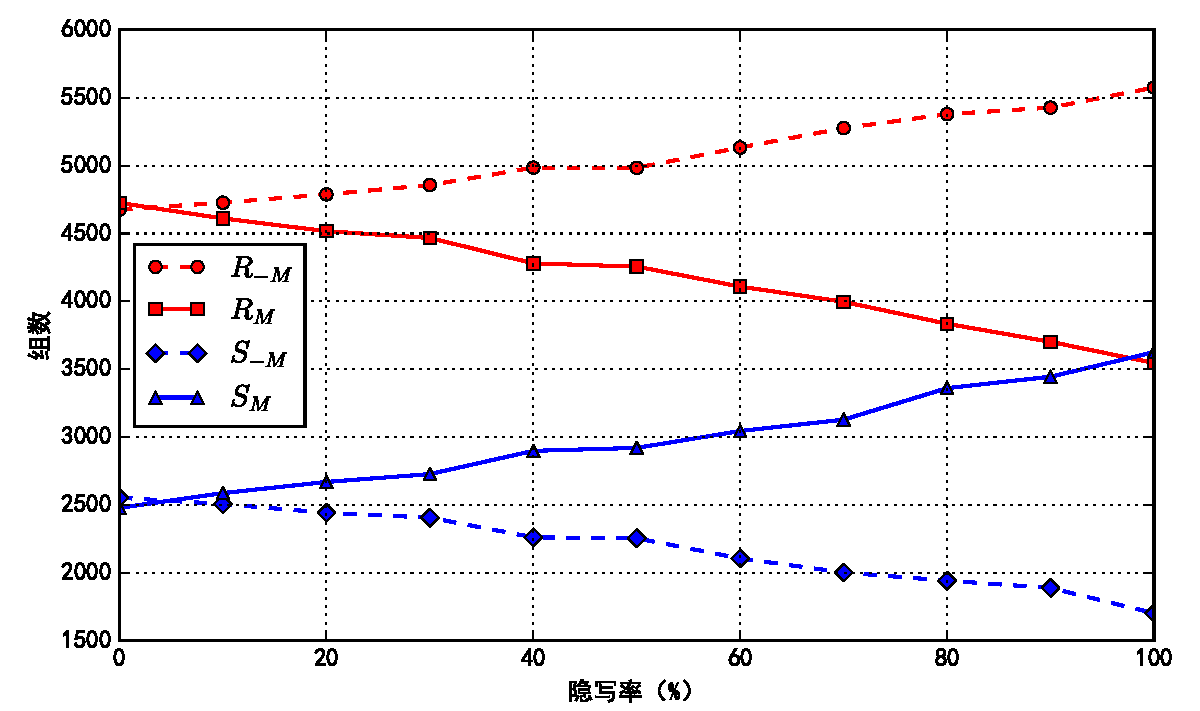
\includegraphics[width=.75\textwidth]{images/rsdemo}
  \end{figure}
\end{frame}

\section{基于SVM的优化}
\subsection{隐写方法设计}
\begin{frame}{可行性与优化目标}
  \begin{block}{应用场景假设}
    \begin{itemize}
      \item 无法获得安全信道交换秘钥
      \item 但可以预先约定少量信息
    \end{itemize}
  \end{block}
  \begin{alertblock}{思考}
    \begin{itemize}
      \item 选择合适的位置(图像块)可以在一定程度上抵抗隐写分析
      \item 根据一些特征判断某个位置是否能安全隐藏消息,实际上是一个SVM分类问题
      \item 隐藏消息的图像块信息也可以作为一个辅助信息隐藏在前几位像素,为了使辅助信息尽量少,选择边长为$\left\lceil {2\sqrt {2l} } \right\rceil$像素的正方形
    \end{itemize}
    \begin{tikzpicture}[scale=.4]
      {\footnotesize
\draw (0,0) rectangle node{消息长度$l$} (5,1);
\draw(5,0) rectangle node{起始坐标$\left(x_0,y_0\right)$}  (10,1);
\draw[fill=gray,fill opacity=0.3](10,0) rectangle node[opacity=1]{$\cdots$}(13,1);
\draw[dashed] (13,0) rectangle node{秘密消息} (23,1);
\draw[fill=gray,fill opacity=0.3](23,0) rectangle node[opacity=1]{$\cdots$}(26,1) ;
\draw [decorate,decoration={brace,amplitude=5pt,mirror}]
(0,0) -- (5,0) node [black,midway,above,sloped,yshift=-14pt]{前$l_1$位};
\draw [decorate,decoration={brace,amplitude=5pt,mirror}] (5,0) -- (10,0) node [black,midway,above,sloped,yshift=-14pt]{接下来$l_2$位};
\filldraw(13,0) circle (2pt) node[below]{$\left(x_0,y_0\right)$};
\draw [decorate,decoration={brace,amplitude=5pt,mirror}] (13,0) -- (23,0) node [black,midway,above,sloped,yshift=-14pt]{$l \times 8$位};
\draw [decorate,decoration={brace,amplitude=5pt},yshift=5pt] (0,1) -- (26,1) node [black,midway,above,sloped,yshift=8pt]{$m \times n$位二进制数据};
}

    \end{tikzpicture}
  \end{alertblock}
\end{frame}

\begin{frame}{引入SVM的隐写系统}
  \centering
  \begin{tikzpicture}[decoration={
	 	markings,
	 	mark=at position 1 with {\arrow[scale=2]{angle 90}};
	 },scale=0.34]
	 
 \path(5,11) node(A) {\bf{发送方}};
 \path(25,11) node(B) {\bf{接收方}};

{\footnotesize
\path<2->  (0,0) node(F) [label=below:SVM分类器]{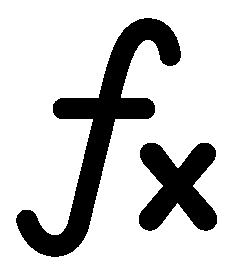
\includegraphics[scale=.09]{icons/function-mathematical-symbol}};
 \path  (0,3) node(M1) [label=below:秘密消息]{
\includegraphics[scale=.08]{icons/email}};
 \path  (0,6) node(C) [label=below:载体] {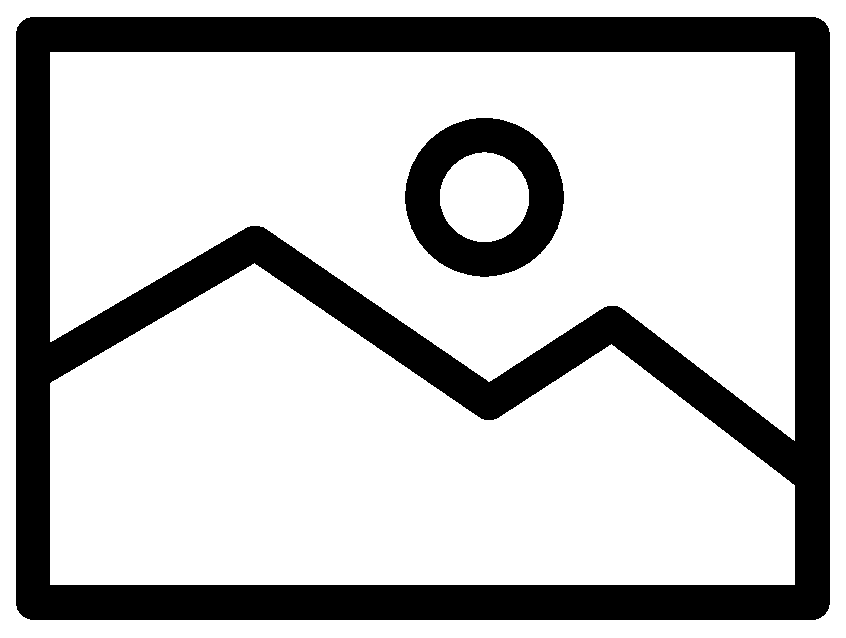
\includegraphics[scale=.04]{icons/landscape-image}};
 \path  (30,3) node(M2) [label=below:秘密消息]{
\includegraphics[scale=.08]{icons/email}};
 \path  (10,3) node(S1) [label=below:伪装图像] {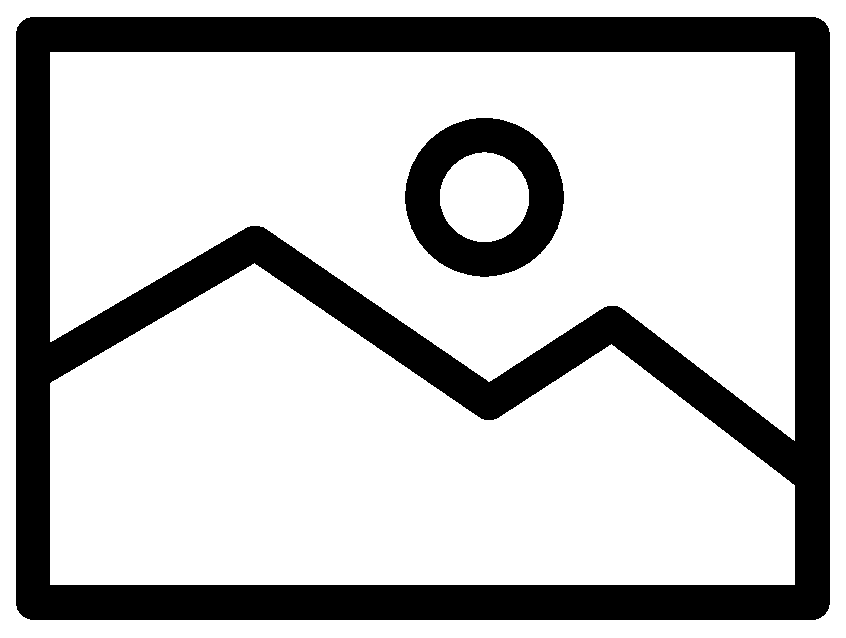
\includegraphics[scale=.04]{icons/landscape-image}};
 \path  (20,3) node(S2) [label=below:伪装图像] {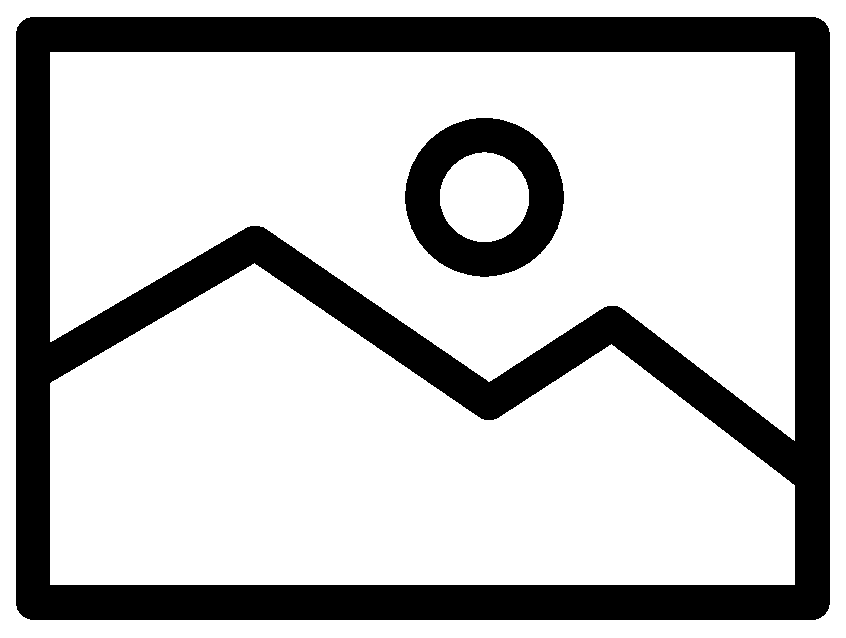
\includegraphics[scale=.04]{icons/landscape-image}};
  \path<3-> (15,8) node(X) [label=above:{约定的$\left(l_1,l_2\right)$}]{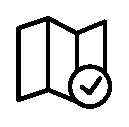
\includegraphics[scale=.4]{icons/map}};
 \draw (3.5,2.1) rectangle node(P1)[align=center] {嵌入消息\\(隐写)} (6.5,3.9);
 \draw (23.5,2.1) rectangle node(P2)[align=center] {提取消息\\(恢复)} (26.5,3.9);
 \draw (13.4,2.5) rectangle node(CH1) {公共信道}
 (16.6,3.5);
  \draw[->,thick] (C) -- (3.4,3.5);
  \draw<2->[->,thick] (F) -- (3.4,2.5);
  \draw[->,thick] (M1) -- (3.4,3);
  \draw[->,thick] (6.6,3) -- (S1);
  \draw[->,thick] (S1)--(13.3,3);
  \draw[->,thick] (16.7,3)--(S2);
  \draw[->,thick] (S2) -- (23.4,3);
  \draw[->,thick] (26.6,3) -- (M2);
  \draw<3->[->,thick] (X) -- (5,4);
  \draw<3->[->,thick] (X) -- (25,4);
  \draw[line width=2,dashed,dash pattern=on 6pt off 4pt,color=gray] (-2,-2) rectangle  (12,10);
  \draw[line width=2,dashed,dash pattern=on 6pt off 4pt,color=gray] (18,-2) rectangle  (32,10);
}

 \end{tikzpicture}
\end{frame}

\subsection{SVM的训练和预测}

\begin{frame}{支持向量机(SVM)}
	\begin{block}{样本集}
		容量为$N$的训练样本集$D = \left\{ {\left( {{{\mathbf{x}}_1},{y_1}} \right),\left( {{{\mathbf{x}}_2},{y_2}} \right), \ldots \left( {{{\mathbf{x}}_N},{y_N}} \right)} \right\}$
		\begin{itemize}
			\item 特征向量${\mathbf{x}_i}$为图像块的特征
			\item 标签$y_i \in \left\{ -1,1\right\}$为安全评估结果,在训练集中由隐写方法评估得到,在使用隐写系统时预测结果作为选择位置的参考指标
		\end{itemize}
	\end{block}

	\begin{alertblock}{SVM分类器}
			\begin{columns}
			\begin{column}{.5\textwidth}
		追求最大“间隔”的分类
		$$
		\begin{aligned}
		\mathop {\max }\limits_{{\mathbf{w}},b} & \quad\frac{2}{{\left\| {\mathbf{w}} \right\|}} \\
		s.t. &\quad {y_i}  \left( {{{\mathbf{w}}^T}{\mathbf{x_i}} + b} \right) \ge 1,i = 1,2, \ldots ,N
		\end{aligned}$$
			\end{column}
					\begin{column}{.41\textwidth}
						过度拟合\&线性不可分
						\begin{itemize}
							\item 核函数:变换特征空间至高维
							\item 软间隔:以权重$C$容忍分类错误
						\end{itemize}
						\end{column}
		\end{columns}
	\end{alertblock}
\end{frame}

\begin{frame}{特征选择}
	\begin{exampleblock}{方差}
		表示图像块像素值的离散程度
		$${\mathop{var}} \left( B \right) = \frac{{\sum\limits_{i = 1}^m {\sum\limits_{j = 1}^n {\left( {{x_{i,j}} - \bar x} \right)} } }}{{m \cdot n - 1}}$$
	\end{exampleblock}

	\begin{alertblock}{整体差异度}
		图像块与整个载体在像素值分布方面的差异
		$${D_{B,I}} =\sum\limits_{i = 0}^{255} {{{\left[ {fre{{\left( B \right)}_i} - fre{{\left( I \right)}_i}} \right]}^2}}$$
		图像块是否“突出”
	\end{alertblock}
\end{frame}

\begin{frame}{特征选择}
	\begin{block}{sc匹配度}
	图像块的LSB平面与秘密消息的LSB平面的匹配程度
	$$sc\_match = \frac{{\sum\limits_{i = 1}^{8l} {p\left( {{M_{Binary}}\left( i \right) = {B_{LSB}}\left( i \right)} \right)} }}{{8l}}$$
	\end{block}

	\begin{exampleblock}{平滑度}
		沿用RS隐写分析中的平滑度定义并加以扩充完善,表示邻接像素之间的差异程度
	,邻接像素为所有方向上的邻接像素
	$${S_i} = \left\{ {x_{i \leftarrow}},{x_{i \to }},{x_{i \uparrow }},{x_{i \downarrow}}\right\}$$
	提出使用\exemple{矩阵偏移}的方法避免重复并提高了计算效率
	$$A{D_ \to } = \left| {B\left( {\left( {1,1} \right),\left( {m,n - 1} \right)} \right) - B\left( {\left( {1,2} \right),\left( {m,n} \right)} \right)} \right|$$
	\end{exampleblock}
\end{frame}




\section{实验与结果}
\subsection{实验环境}
\begin{frame}{实验平台和设置}
	\begin{description}
		\item[Windows10] 操作系统
		\item[MATLAB2015b] 主要的图像处理、数据计算平台和语言
		\item[Python3.5] 完成了一些数据预处理、收集和绘制图像的任务
		\item[UCID] 图像数据集,包含1338张彩色图像,为方便处理在实验中全部转换为灰度图像
	\end{description}
	\begin{block}{}
		\begin{itemize}
			\item 训练阶段使用嵌入率为5\%-50\%的2000个图像块(在图像数据集中随机抽样)样本训练不同参数的SVM,并使用200个图像样本作为检验集进行调整
			\item
			预测阶段使用嵌入率分别为5\%-50\%(步长5\%)的13380样本(1338张图像,每张10个位置)验证SVM的分类准确率,隐写系统在安全方面的提升依赖于SVM的预测准确率。
		\end{itemize}
	\end{block}
\end{frame}

\subsection{实验结果}
\begin{frame}{SVM的训练}
	使用80组不同参数进行训练,得到的SVM在错误率方面的表现
	\begin{figure}
		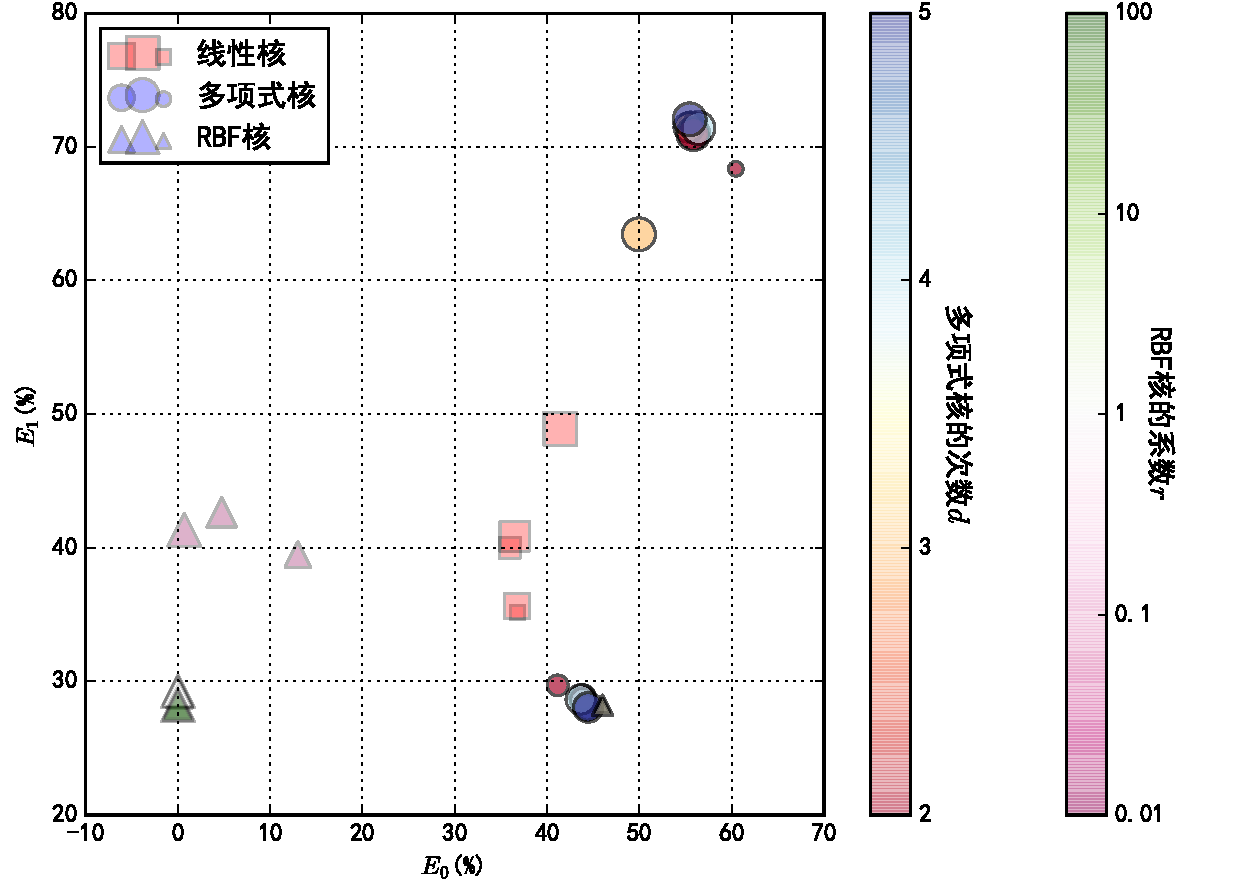
\includegraphics[width=.9\textwidth]{images/scatter}
	\end{figure}
\end{frame}

\begin{frame}{挑选6组性质典型的SVM}
	% Table generated by Excel2LaTeX from sheet 'Sheet1'
{\small
\begin{table}[htbp]
  \centering
  \caption{6组SVM的参数}
    \begin{tabular}{cccccccc}
    \toprule
    {编号} & {核类型} & {代价$C$} & {次数$d$} & {系数$\gamma$} & {训练错误率$E_0$} & {检验错误率$E_1$} & {支持向量数} \\
    \midrule
    1     & \multirow{2}[1]{*}{线性核} & 0.01  & \multirow{2}[1]{*}{1} & 1     & 36.8  & 35.15 & 1566 \\
    2     &       & 1     &       & 1     & 36.75 & 35.65 & 1045 \\ \midrule
    3     & \multirow{3}[0]{*}{多项式核} & 0.1   & 2     & 1     & 41.15 & 29.7  & 208 \\
    4     &       & 0.1   & 4     & 1     & 43.8  & 28.65 & 90 \\
    5     &       & 10    & 4     & 0.1   & 43.65 & 28.65 & 83 \\ \midrule
    6     & RBF核  & 1     & 无穷大   & 1     & 0.2   & 28.95 & 2000 \\
   \bottomrule
    \end{tabular}%
  \label{tab:addlabel}%
\end{table}%
}

\end{frame}

\begin{frame}{对抗RS隐写分析}
	\begin{figure}
		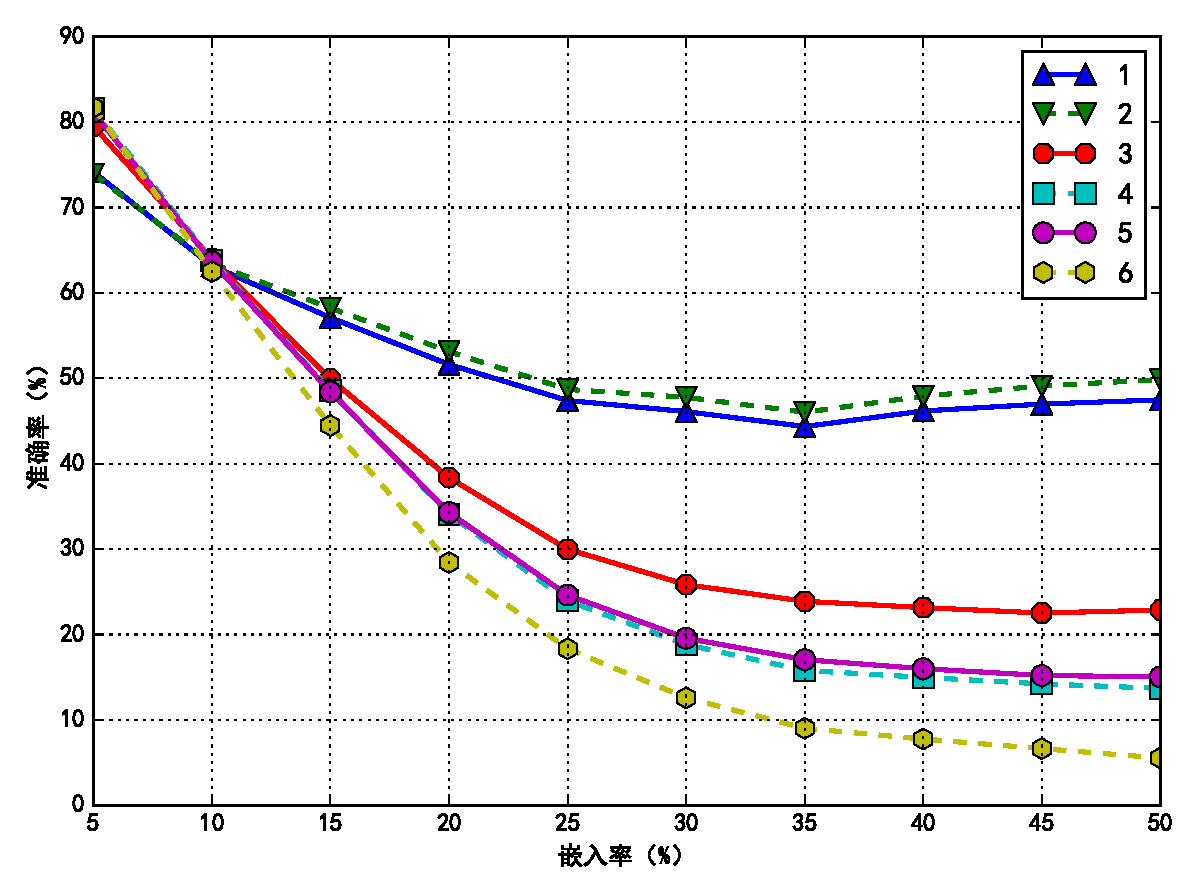
\includegraphics[width=.9\textwidth]{images/rs_prediction}
	\end{figure}
\end{frame}

\begin{frame}{对抗SPA}
	\begin{figure}
		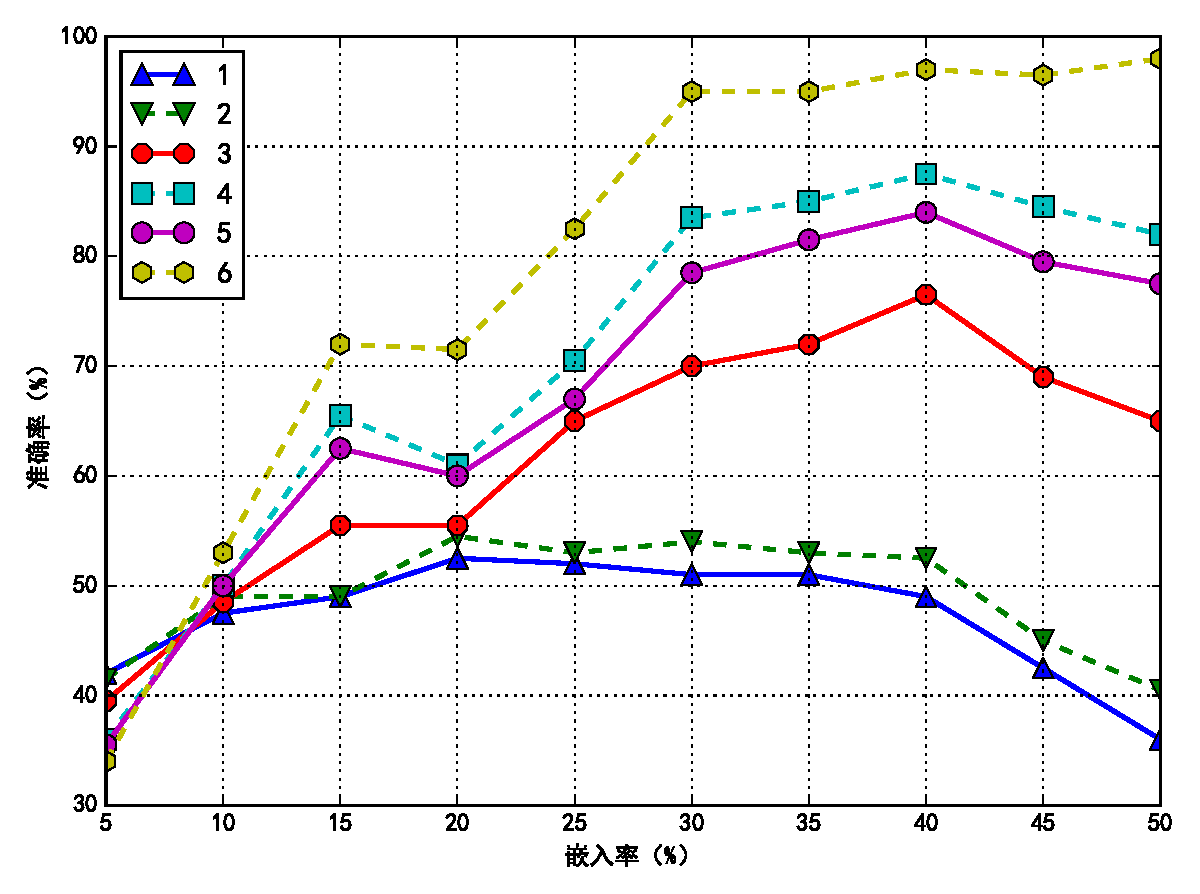
\includegraphics[width=.9\textwidth]{images/spaprediction}
	\end{figure}
\end{frame}

\begin{frame}{$\chi^2$测验}
	\begin{figure}
		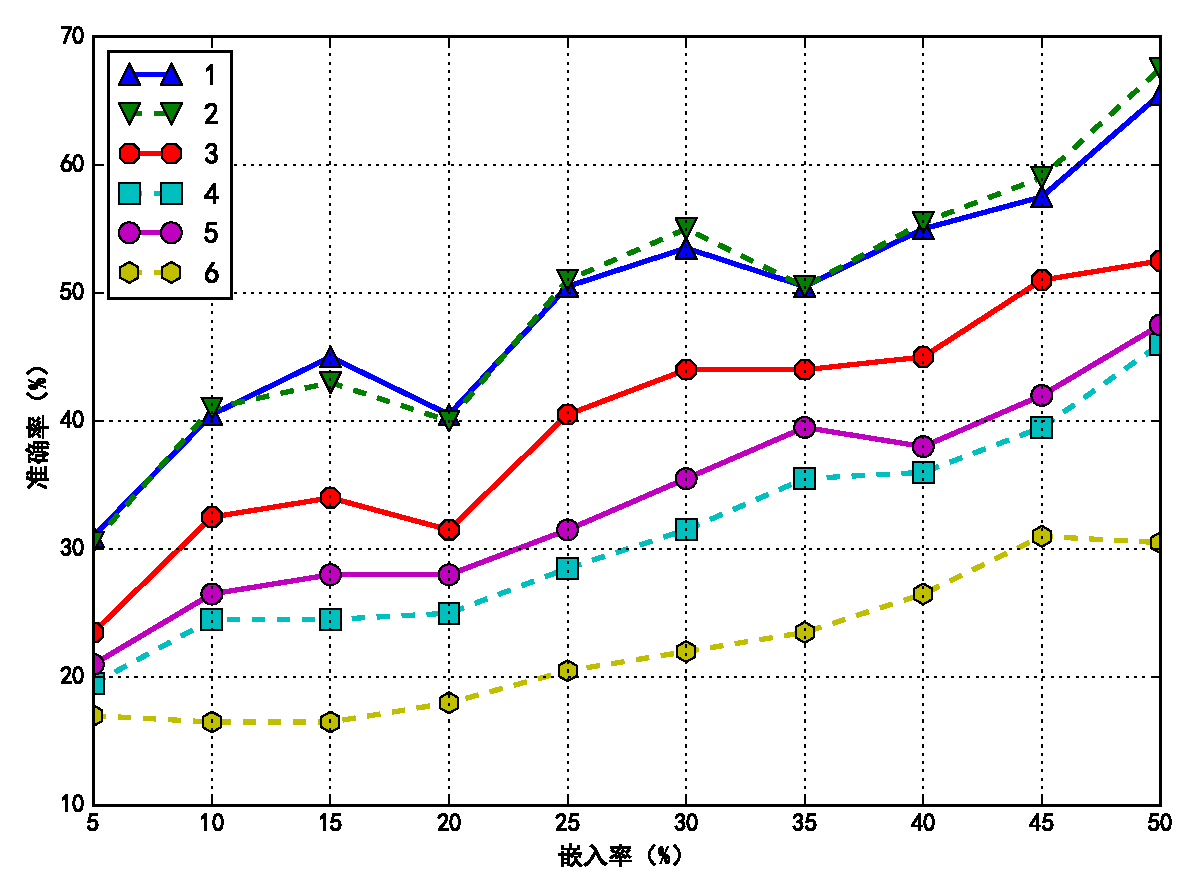
\includegraphics[width=.9\textwidth]{images/chi2prediction}
	\end{figure}
\end{frame}

\begin{frame}{Thanks}
	\centering
	论文中用到的全部源代码(包括本幻灯片),数据,图像,文档见\\
	\faChain \url{https://github.com/Lixinyi-DUT/graduation-project}
\end{frame}

\end{document}
